\documentclass{article}

%Colors
\usepackage[dvipsnames]{xcolor}

%Basics
\usepackage[margin=1in]{geometry}
\usepackage{amsmath, amssymb, amsthm}
\usepackage{enumitem}

%Creating Subfigures
\usepackage{subcaption}

%Creating Graphs
\usepackage{tikz}
\usepackage{pgfplots} \pgfplotsset{compat=newest}
\usetikzlibrary{angles, quotes}
\usepgflibrary{shapes}
\usetikzlibrary{positioning}
    % Define a counter
    \newcount\CircNum
    % Macro to hold a color name
    \newcommand\Clr{black}

% Fixes issues with underline wrapping, don't worry about it
\usepackage{soul}

%Formatting and Spacing
\setitemize[1]{noitemsep, parsep = 5pt, topsep = 5pt}
\setenumerate[1]{label = (\alph*), parsep = 1pt, topsep = 5pt}
\setlength\parindent{0pt}
\linespread{1.1}

%Easy Numbering
\newcounter{counter}
\newcommand{\Exercise}{Exercise \stepcounter{counter}\thecounter}

%Cases Environment (Messy)
\newlist{Cases}{enumerate}{3}
\setlist[Cases]{leftmargin = .25in, label = {Case \arabic*.}, topsep = 0.01in, itemsep = 0.04in, itemindent = .5in, parsep = 0in}

%Custom Title Fields
\newcommand{\hmwkTitle}{Homework 8 (with Solutions)}
\newcommand{\hmwkDueDate}{April 19, 2022}
\newcommand{\hmwkClass}{Honors Discrete Mathematics}
\newcommand{\hmwkClassInstructor}{Gerandy Brito}
\newcommand{\hmwkSection}{Spring 2022}
\newcommand{\hmwkAuthorName}{Sarthak Mohanty}

%Headers and Footers
\usepackage{fancyhdr}
\usepackage{extramarks}
\pagestyle{fancy}
\lhead{\hmwkAuthorName}
\chead{\hmwkClass \ (\hmwkClassInstructor)}
\rhead{Homework 8}
\cfoot{\thepage}
\renewcommand\headrulewidth{0.4pt}
\renewcommand\footrulewidth{0.4pt}

\title{
    \vspace{2in}
    \textbf{\hmwkClass:\\ \hmwkTitle}\\
    \normalsize\vspace{0.1in}\small{Due\ on\ \hmwkDueDate\ at 11:59pm}\\
    \vspace{0.1in}\large{\textit{\hmwkClassInstructor\ \hmwkSection}}
    \vspace{3in}
    \author{\textbf{\hmwkAuthorName}}
    \date{}
}

\begin{document}

\maketitle
\pagebreak

\subsection*{\Exercise}
    \textit{(Combinations with Repetition) } For each part, use the ``stars and bars" method discussed in class.
    \begin{enumerate}
        \item How many integer-valued solutions are there to the equation $$x_{1} + x_{2} + x_{3} + x_{4} + x_{5} = 47$$ given that $x_{1}, x_{2} > 0$ and $x_{3}, x_{4}, x_{5} \ge 10$?
        \item Consider the two sets $X = \{1, 2, 3, 4, 5\}$ and $Y = \{6, 7, 8, 9, 10\}$. How many possible functions $f : X \rightarrow Y$ are there such that if $i < j$ then $f(i) \le f(j)$? % monotoniciticy next time
        \item Stefan throws a fair six-sided die five times. Letting the outcome of the $n$th throw be $a_{n}$, how many cases are there such that $a_{1} < a_{2} < a_{3} \le a_{4} \le a_{5}$?
    \end{enumerate}

\subsection*{Solution}
    \begin{enumerate}
        \item We begin by partitioning $1$ for $x_{1}, x_{2}$. Furthermore, we partition $10$ for $x_{3}, x_{4}, x_{5}$. Then we have the equation $$x_{1} + x_{2} + x_{3} + x_{4} + x_{5} = 47 - 2 - 30 = 15.$$ We can think of counting the integer solutions to the equation above as counting strings over an alphabet consisting of a divider $|$ (i.e.\ ``bar") and identical objects $\star$ (i.e.\ ``stars"). In this case, we must choose $(5 - 1) = 4$ dividers over a string of length $15 + 4 = 19$. Hence our answer is given by $$\binom{15 + 4}{4} = \binom{19}{4} = 3876.$$
        \item This problem is equivalent to finding the number of ways to choose $5$ numbers from $Y$ with repetition. Every such selection of five numbers from $Y$ corresponds to a unique function $f \colon X \rightarrow Y$ that satisfies our conditions. Again using ``stars and bars", the number of ways to choose these five numbers from $Y$ with repetition is $$\binom{5 + 5 - 1}{5} = \binom{9}{5} = 126.$$
        \item First find the number of cases such that $a_{1} \le a_{2} \le a_{3} \le a_{4} \le a_{5}$. This is equivalent to choosing $5$ numbers from $1$ to $6$ with repetition, since there is one arrangement satisfying the given condition per one selection. Using ``stars and bars", the number of ways to do this is $$\binom{6 + 5 - 1}{5} = \binom{10}{5} = 252.$$ Now, let $A$ be the set of cases where $a_{1} = a_{2} \le a_{3} \le a_{4} \le a_{5}$, and $B$ the set of cases such that $a_{1} \le a_{2} = a_{3} \le a_{4} \le a_{5}$. The number of elements in $A$ is equivalent to the number of cases when choosing $4$ numbers out of $1$ through $6$ with repetition, as we can consider $a_{1}$ and $a_{2}$ as a single number. The number of ways to do this is $$\binom{6 + 4 - 1}{4} = \binom{9}{4} = 126.$$ Likewise, the number of elements in $B$ is also $126$.
        
        \vspace{1.5mm}
        Next we find $|A \cap B|$, which is the number of cases where $a_{1} = a_{2} = a_{3} \le a_{4} \le a_{5}$. For a similar reason as above, we can deduce that $$|A \cap B| = \binom{6 + 3 - 1}{3} = \binom{8}{3} = 56.$$ Finally using PIE, the answer is $$252 - (126 + 126 - 56) = 56.$$
    \end{enumerate}

\subsection*{\Exercise}
    \textit{(Twelve Knights of the Round Table)} In this story, we focus on a $13$ person round table, composed of King Arthur and his twelve knights. Show your work for each part.
    \begin{enumerate}
        \item King Arthur calls for an urgent meeting with his knights. They are about to sit around the round table, when the king mentions that he will like to sit next to Sir Lancelot. In how many ways can they all sit? Two sittings are considered different if at least one knight has a different neighbor to the left or a different neighbor to the right.
        \item The king and his knights have all taken their seats. However, one of King Arthur's $12$ knights, the traitorous Sir Mordred, plans to poison four others at the table. To avoid suspicion, he will not poison two people adjacent to each other on the table. How many ways can he poison the others?
        
        \vspace{1mm}\textit{Note: Sir Mordred would prefer not to poison himself.}
        \item King Arthur discovers Mordred's treachery, and strips him of his title. \ul{There are now $11$ knights (plus King Arthur) sitting around a $12$ person round table.}
        
        \vspace{1.5mm} \qquad Now, King Arthur is holding a piece of gold. For simplicity, let us label him $+1$. As the other knights are not holding gold, we will label them $-1$. Merlin, the magician, has the power to switch the sign of the numbers in any $k$ consecutive sequence of people. Is it possible to ``shift'' the only piece of gold to a knight adjacent to King Arthur if 
        \begin{enumerate}[label = \roman*.]
            \item $k = 4$?
            \item $k = 5$?
        \end{enumerate}
        
        \vspace{1mm}\textit{Hint: This problem does not require much combinatorical knowledge. Furthermore, we briefly covered a topic known as \textbf{invariants} early on in the semester...}
    \end{enumerate}
    
\subsection*{Solution}
    \begin{enumerate}
        \item Due to rotational symmetry, there is only one choice for King Arthur. There are two choices for Sir Lancelot, and for each of those choices, there are $(13 - 2)! = 11!$ ways to arrange the remaining knights. Hence our answer is $2 \times 11!$.
        \item Since Sir Mordred does not poison himself, we can reduce the problem to poisoning four non-consecutive royals in a \underline{line} of length $12$. Note that if four royals are poisoned, that leaves $12 - 4 = 8$ royals not poisoned. Representing these using $\mid$ (``bars"), we have $$| \quad | \quad | \quad | \quad | \quad | \quad | \quad |$$ Now any poisoned royals must be nonconsecutive, so any two poisoned royals must have a non-poisoned royal between them. Hence there are $8 + 1$ possibilities for a poisoned royal to sit. Representing these possibilities using $\bigcirc$, we now have $$\bigcirc \quad | \quad \bigcirc \quad | \quad \bigcirc \quad | \quad \bigcirc \quad | \quad \bigcirc \quad | \quad \bigcirc \quad | \quad \bigcirc \quad | \quad \bigcirc \quad | \quad \bigcirc$$ Mordred must choose $4$ of these $9$ royals to poison. Each of these combinations uniquely determines a natural ordering. For example, if Mordred poisons the first four possible royals, the ordering is given as
        $$\star_{1} \quad |_{2} \quad \star_{3} \quad |_{4} \quad \star_{5} \quad |_{6} \quad \star_{7} \quad |_{8} \quad \bigcirc \quad |_{9} \quad \bigcirc \quad |_{10} \quad \bigcirc \quad |_{11} \quad \bigcirc \quad |_{12} \quad \bigcirc$$
        To summarize, there are $12 - 4 + 1$ possibilities, and we must choose $4$ of them. Hence our answer is given by $$\binom{12 - 4 + 1}{4} = \binom{9}{4} = 126.$$
        
        \vspace{1mm}
        \textbf{Remark.} Note that our explanation can be generalized. The number of ways to choose $k$ non-consecutive objects from $n$ consecutive terms is $\binom{n - k + 1}{k}$.
        \item 
        \begin{enumerate}[label = \roman*.]
            \item No, not possible. Select a subset of people which satisfies the condition that there are evenly many selected people among any $k$ successive ones, as shown in Figure \ref{fig:1}. For our invariant we take the product of the numbers on the selected people, call it $P$. Initially, it equals $-1$, but if the $+1$ has been ``shifted" to the right adjacent knight which is not among those selected, it is $1$. Since switching the sign of the numbers in any $k$ consecutive sequence of people does not change $P$, we conclude that we will never be able to get to the right adjacent knight. A similar argument follows for the left adjacent knight.
            \begin{figure}[htbp]
            \centering
            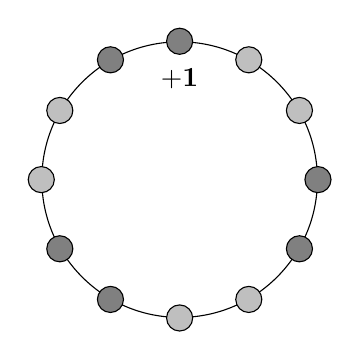
\begin{tikzpicture}
                % draw the main circle
                \node [circle, draw, minimum size=3.5cm] (c) {};
                
                \foreach \a in {1,2,...,12}{
                  % if \a is equal to \CircNum, set the color to blue
                  % otherwise set it to black
                  \ifnum\ifnum\a=3 1\else\ifnum\a=4 1\else\ifnum\a=7 1\else\ifnum\a=8 1\else\ifnum\a=11 1\else\ifnum\a=12 1\else0 \fi\fi\fi\fi\fi\fi =1 %
                      \renewcommand\Clr{gray}
                  \else
                      \renewcommand\Clr{gray!50}
                  \fi
                  % make a new node for the small circles
                  \node[ draw, % draw the outline
                         fill = {\Clr}, % fill it with the color defined by the macro
                         minimum size=2mm, % set the size
                         circle, % circular shape
                         ] at (c.\a*360/12) % position it on the edge of the main circle
                         (n\a) {};
                }
                \node[below = 0.5mm of n3] {$\mathbf{+1}$};
            \end{tikzpicture}
            \caption{An illustration of our invariant. Darkened vertices are selected.}
            \label{fig:1}
            \end{figure}
            
            \item Yes, it is possible. Below is a possible sequence of transformations that Merlin could have used to shift the piece of gold to the knight left-adjacent to the king. Note that unlike part (a), darkened vertices represent $+1$ here.
            \begin{figure}[htbp]
            \centering
            
            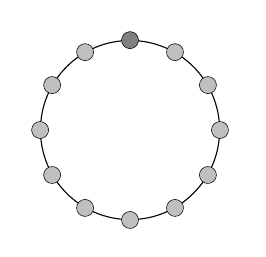
\begin{tikzpicture}[remember picture, scale = 0.65, transform shape]
                \node [circle, draw, minimum size=3.5cm] (c) {};
                \foreach \a in {1,2,...,12}{
                  \ifnum\a=3
                      \renewcommand\Clr{gray}
                  \else
                      \renewcommand\Clr{gray!50}
                  \fi
                  \node[black, draw, very thin, fill = {\Clr}, minimum size=2mm, circle,] at (c.\a*360/12) (n\a) {};
                }
                \useasboundingbox (-2,0) rectangle (2.1,2);
                \path (current bounding box.north east) -- (current bounding box.south east) coordinate[midway] (1BL);
            \end{tikzpicture}
            \hspace*{0.5cm}
            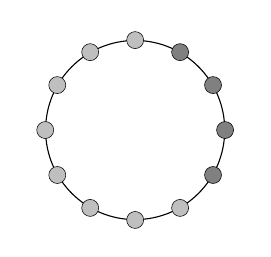
\begin{tikzpicture}[remember picture, scale = 0.65, transform shape]
                \node [circle, draw, minimum size=3.5cm] (c) {};
                \foreach \a in {1,2,...,12}{
                  \ifnum\ifnum\a=2 1\else\ifnum\a=1 1\else\ifnum\a=12 1\else\ifnum\a=11 1\else0 \fi\fi\fi\fi =1 %
                      \renewcommand\Clr{gray}
                  \else
                      \renewcommand\Clr{gray!50}
                  \fi
                  \node[black, draw, very thin, fill = {\Clr}, minimum size=2mm, circle,] at (c.\a*360/12) (n\a) {};
                }
                \useasboundingbox (-2.1,0) rectangle (2.1,2);
                \path (current bounding box.north west) -- (current bounding box.south west) coordinate[midway] (1BR);
                \path (current bounding box.north east) -- (current bounding box.south east) coordinate[midway] (2BL);
            \end{tikzpicture}
            \hspace*{0.5cm}
            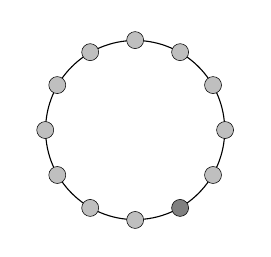
\begin{tikzpicture}[remember picture, scale = 0.65, transform shape]
                \node [circle, draw, minimum size=3.5cm] (c) {};
                
                \foreach \a in {1,2,...,12}{
                  \ifnum\a=10 %
                      \renewcommand\Clr{gray}
                  \else
                      \renewcommand\Clr{gray!50}
                  \fi
                  \node[black, draw, very thin, fill = {\Clr}, minimum size=2mm, circle,] at (c.\a*360/12) (n\a) {};
                }
                \useasboundingbox (-2.1,0) rectangle (2.1,2);
                \path (current bounding box.north west) -- (current bounding box.south west) coordinate[midway] (2BR);
                \path (current bounding box.north east) -- (current bounding box.south east) coordinate[midway] (3BL);
                \end{tikzpicture}
            \hspace*{0.5cm}
            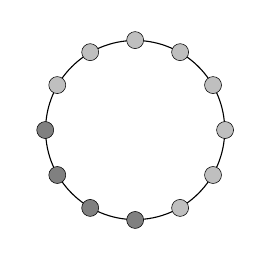
\begin{tikzpicture}[remember picture, scale = 0.65, transform shape]
                \node [circle, draw, minimum size=3.5cm] (c) {};
                
                \foreach \a in {1,2,...,12}{
                  \ifnum\ifnum\a=9 1\else\ifnum\a=8 1\else\ifnum\a=7 1\else\ifnum\a=6 1\else0 \fi\fi\fi\fi =1 %
                      \renewcommand\Clr{gray}
                  \else
                      \renewcommand\Clr{gray!50}
                  \fi
                  \node[black, draw, very thin, fill = {\Clr}, minimum size=2mm, circle,] at (c.\a*360/12) (n\a) {};
                }
                \useasboundingbox (-2.1,0) rectangle (2,2);
                \path (current bounding box.north west) -- (current bounding box.south west) coordinate[midway] (3BR);
            \end{tikzpicture}
            \tikz[overlay,remember picture]{\draw[-latex,thick] (1BL) -- (1BL-|1BR)}
            \tikz[overlay,remember picture]{\draw[-latex,thick] (2BL) -- (2BL-|2BR)}
            \tikz[overlay,remember picture]{\draw[-latex,thick] (3BL) -- (3BL-|3BR)}
            
            \vspace{3mm}
            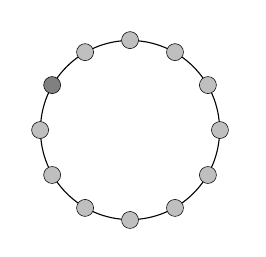
\begin{tikzpicture}[remember picture, scale = 0.65, transform shape]
                \node [circle, draw, minimum size=3.5cm] (c) {};
                
                \foreach \a in {1,2,...,12}{
                  \ifnum\a=5 %
                      \renewcommand\Clr{gray}
                  \else
                      \renewcommand\Clr{gray!50}
                  \fi
                  \node[black, draw, very thin, fill = {\Clr}, minimum size=2mm, circle,] at (c.\a*360/12) (n\a) {};
                }
                \useasboundingbox (-2,0) rectangle (2.1,2);
                \path (current bounding box.north east) -- (current bounding box.south east) coordinate[midway] (4BL);
            \end{tikzpicture}
            \hspace*{0.5cm}
            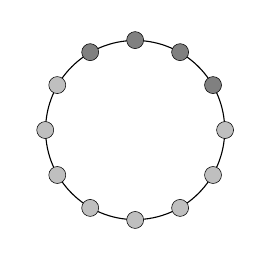
\begin{tikzpicture}[remember picture, scale = 0.65, transform shape]
                \node [circle, draw, minimum size=3.5cm] (c) {};
                
                \foreach \a in {1,2,...,12} {
                  \ifnum\ifnum\a=4 1\else\ifnum\a=3 1\else\ifnum\a=2 1\else\ifnum\a=1 1\else0 \fi\fi\fi\fi =1 %
                      \renewcommand\Clr{gray}
                  \else
                      \renewcommand\Clr{gray!50}
                  \fi
                  \node[black, draw, very thin, fill = {\Clr}, minimum size=2mm, circle,] at (c.\a*360/12) (n\a) {};
                }
                \useasboundingbox (-2.1,0) rectangle (2.1,2);
                \path (current bounding box.north west) -- (current bounding box.south west) coordinate[midway] (4BR);
                \path (current bounding box.north east) -- (current bounding box.south east) coordinate[midway] (5BL);
            \end{tikzpicture}
            \hspace*{0.5cm}
            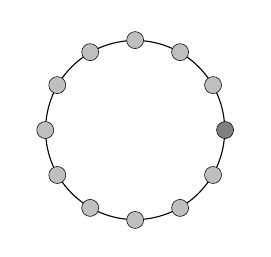
\begin{tikzpicture}[remember picture, scale = 0.65, transform shape]
                \node [circle, draw, minimum size=3.5cm] (c) {};
                
                \foreach \a in {1,2,...,12}{
                  \ifnum\a=12 %
                      \renewcommand\Clr{gray}
                  \else
                      \renewcommand\Clr{gray!50}
                  \fi
                  \node[black, draw, very thin, fill = {\Clr}, minimum size=2mm, circle,] at (c.\a*360/12) (n\a) {};
                }
                \useasboundingbox (-2.1,0) rectangle (2.1,2);
                \path (current bounding box.north west) -- (current bounding box.south west) coordinate[midway] (5BR);
                \path (current bounding box.north east) -- (current bounding box.south east) coordinate[midway] (6BL);
            \end{tikzpicture}
            \hspace*{0.5cm}
            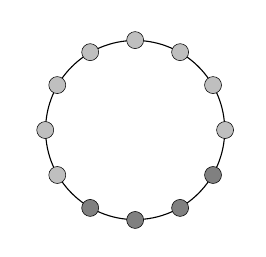
\begin{tikzpicture}[remember picture, scale = 0.65, transform shape]
                \node [circle, draw, minimum size=3.5cm] (c) {};
                
                \foreach \a in {1,2,...,12} {
                  \ifnum\ifnum\a=11 1\else\ifnum\a=10 1\else\ifnum\a=9 1\else\ifnum\a=8 1\else0 \fi\fi\fi\fi =1 %
                      \renewcommand\Clr{gray}
                  \else
                      \renewcommand\Clr{gray!50}
                  \fi
                  \node[black, draw, very thin, fill = {\Clr}, minimum size=2mm, circle,] at (c.\a*360/12) (n\a) {};
                  \useasboundingbox (-2.1,0) rectangle (2,2);
                  \path (current bounding box.north west) -- (current bounding box.south west) coordinate[midway] (6BR);
                }
            \end{tikzpicture}
            \tikz[overlay,remember picture]{\draw[-latex,thick] (4BL) -- (4BL-|4BR)}
            \tikz[overlay,remember picture]{\draw[-latex,thick] (5BL) -- (5BL-|5BR)}
            \tikz[overlay,remember picture]{\draw[-latex,thick] (6BL) -- (6BL-|6BR)}
            
            \vspace{3mm}
            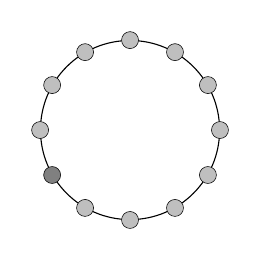
\begin{tikzpicture}[remember picture, scale = 0.65, transform shape]
                \node [circle, draw, minimum size=3.5cm] (c) {};
                \foreach \a in {1,2,...,12}{
                  \ifnum\a=7
                      \renewcommand\Clr{gray}
                  \else
                      \renewcommand\Clr{gray!50}
                  \fi
                  \node[black, draw, very thin, fill = {\Clr}, minimum size=2mm, circle,] at (c.\a*360/12) (n\a) {};
                }
                \useasboundingbox (-2,0) rectangle (2.1,2);
                \path (current bounding box.north east) -- (current bounding box.south east) coordinate[midway] (7BL);
            \end{tikzpicture}
            \hspace*{0.5cm}
            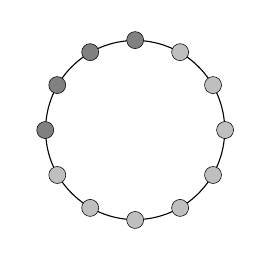
\begin{tikzpicture}[remember picture, scale = 0.65, transform shape]
                \node [circle, draw, minimum size=3.5cm] (c) {};
                \foreach \a in {1,2,...,12} {
                  \ifnum\ifnum\a=6 1\else\ifnum\a=5 1\else\ifnum\a=4 1\else\ifnum\a=3 1\else0 \fi\fi\fi\fi =1 %
                      \renewcommand\Clr{gray}
                  \else
                      \renewcommand\Clr{gray!50}
                  \fi
                  \node[black, draw, very thin, fill = {\Clr}, minimum size=2mm, circle,] at (c.\a*360/12) (n\a) {};
                  \useasboundingbox (-2.1,0) rectangle (2.1,2);
                    \path (current bounding box.north west) -- (current bounding box.south west) coordinate[midway] (7BR);
                    \path (current bounding box.north east) -- (current bounding box.south east) coordinate[midway] (8BL);
                }
            \end{tikzpicture}
            \hspace*{0.5cm}
            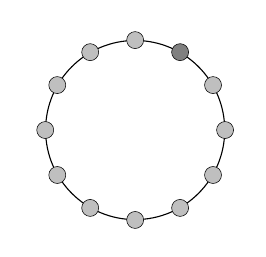
\begin{tikzpicture}[remember picture, scale = 0.65, transform shape]
                \node [circle, draw, minimum size=3.5cm] (c) {};
                \foreach \a in {1,2,...,12}{
                  \ifnum\a=2 %
                      \renewcommand\Clr{gray}
                  \else
                      \renewcommand\Clr{gray!50}
                  \fi
                  \node[black, draw, very thin, fill = {\Clr}, minimum size=2mm, circle,] at (c.\a*360/12) (n\a) {};
                    \useasboundingbox (-2.1,0) rectangle (2,2);
                    \path (current bounding box.north west) -- (current bounding box.south west) coordinate[midway] (8BR);
                }
            \end{tikzpicture}
            \tikz[overlay,remember picture]{\draw[-latex,thick] (7BL) -- (7BL-|7BR)}
            \tikz[overlay,remember picture]{\draw[-latex,thick] (8BL) -- (8BL-|8BR)}
            
            \vspace{3mm}
            \caption{A possible series of transformations}
            \label{E2cii}
            \end{figure}
            
        \end{enumerate}
        
    \end{enumerate}

\subsection*{\Exercise}
    \textit{(PHP: Introduction)} In your explanations for this problem, clearly state your pigeons and your pigeonholes.
    \begin{enumerate}
        \item Fifteen girls ate 100 berries. Prove that some pair of girls ate an identical number of berries.
        \item There are 82 berries of various types. Prove that you can either pick ten berries, each of different types, or ten berries of the same type.
        \item You are given 11 different natural numbers, none greater than 20. Prove that two of these can be chosen, one of which divides the other.
    \end{enumerate}

\subsection*{Solution}
    \begin{enumerate}
        \item Suppose each girl ate a different number of berries. Then the number of berries the girls ate is at least $0 + 1 + 2 + \dots + 14 = 105$. There are $105$ pigeons (the number of berries each girl ate) and $100$ holes (the maximum number of berries the girls can eat), so by the pigeonhole principle, two pigeons must be in the same hole. It follows that two girls must have eaten an identical number of berries.
        
        \vspace{1mm}
        \textbf{Remark.} Making the assumption that a girl must eat at least one berry, and instead summing the numbers from $1$ to $15$ is also acceptable.
        \item If there are at least ten berries of the same type, then our work is done. Hence, suppose there are not ten berries of any one type. Then there are at most $9$ berries of each type. Letting our pigeons be the berries and the pigeonholes be the number of berries of each type, we see that by the pigeonhole principle, there must be at least $\lceil \frac{82}{9} \rceil = 10$ different types of berries.
        \item We can divide the numbers from $1$ through $20$ into ten disjoint sets, such that if a pair of numbers is elected from the same set, one of the pair divides the other: $$\{11\}, \{13\}, \{15\}, \{17\}, \{19\}, \{1, 2, 4, 8, 16\}, \{3, 6, 12\}, \{5, 10, 20\}, \{7, 14\}, \{9, 18\}.$$ Then, of any eleven numbers not greater than $20$ (the pigeons), two of them must fit in one of these pigeonholes, and thus one of these two divides the other.
        %%%NEXT TIME: Ask if it is possible, don't give the result.
    \end{enumerate}

\subsection*{\Exercise}
    \textit{(PHP: Visualizations)} For these pigeonhole principle problems, include drawings to support your answer.
    \begin{enumerate}
        \item Given seven points inside a regular hexagon with side length 1, prove that there exists two points with distance at most 1. 
        \item In a cube of side length 9 there are 1500 points. Prove that there exist two points situated at distance at most 1 from each other.
        
        \vspace{1mm} \textit{Note: Your drawing for this part just needs to get the main idea across.}
        \item Six points are chosen inside a $3 \times 4$ rectangle. Prove that a pair of them can be chosen such that the distance between them is at most $\sqrt{5}$.
        
        \vspace{1mm} \textit{Note: This one is tough. Don't be discouraged if it takes a long time!}
    \end{enumerate}

\subsection*{Solution}
    \begin{enumerate}
        \item Divide the hexagon into six equilateral triangles, each with side length $1$, as shown in Figure \ref{fig:E4a}. By the pigeonhole principle, there must be at least $\lceil \frac{7}{6} \rceil = 2$ points in the same triangle. The maximum distance between two points in any of these equilateral triangles is $1$, and thus we are done.
        \item \qquad Assume there are no such two points. By the Kepler conjecture, optimally arranged spheres will occupy at most $10^{3} \times \frac{\pi}{3\sqrt{2}} \approx 740$ units of volume inside a cube of side length $10$. However, the volume of $1500$ spheres with radius $\frac{1}{2}$ is $1500 \times \frac{4}{3}\pi(\frac{1}{2})^{3} \approx 785$. By the pigeonhole principle, there must be at least $2$ spheres that share some volume. Now each sphere can be uniquely mapped to a point (by its center). As the distance between any two centers is $\frac{1}{2} + \frac{1}{2} = 1$, there must be two points that are a distance of at most $1$ from each other. 
        
        \vspace{1.5mm}
        \qquad Note that we use a cube of side length $10$ instead of $9$ in our calculations. This is because points near the edges of the $9 \times 9 \times 9$ cube can map to spheres extending up to $\frac{1}{2}$ units past the cube.
        
        \vspace{1.5mm}
        \qquad To confirm this statement, I attempted to pack these spheres in such a cube in Mathematica. The results are displayed in Figure \ref{fig:E3b}. As expected, less than $1500$ spheres were able to fit. 
        
        \vspace{1.5mm}
        \textcolor{red}{\textbf{Remark.}} As the solution utilized tools outside the scope of this course, all students were awarded full credit for this part.
        
        \begin{figure}[htbp]
            \centering
            \begin{minipage}{.45\textwidth}
                \centering
                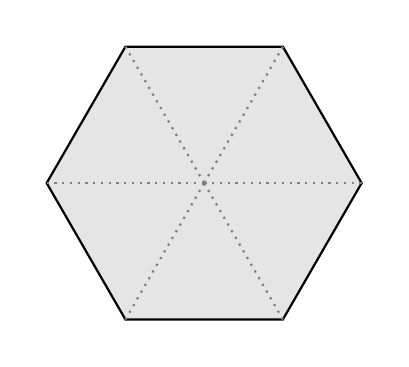
\begin{tikzpicture}[scale=1]
                    \node (A) [draw,thick,regular polygon, regular polygon sides=6, minimum     size=4cm,outer sep=0pt,fill=gray!20] {};
                    
                    \foreach \V [count=\Vi from 1] in {D,E,F,A,B,C}                           {\node at (A.corner \Vi) [anchor=360/6*(\Vi-1))+270] {}; }
                    \coordinate [label=above:\textcolor{blue}{}] (C) at (.2, .2);
                    
                    \foreach \i in {1,...,6} {
                        \draw[gray,thick, dotted] (A.corner \i) -- (A.center);
                    }
                \end{tikzpicture}
                \caption{Illustration of E4 part (a)}
                \label{fig:E4a}
            \end{minipage}
            \begin{minipage}{.45\textwidth}
                \centering
                
\includegraphics[scale = 0.3]{Homework/Homework 8 Files/E4b.pdf}
                \caption{Illustration of E4 part (b)}
                \label{fig:E3b}
            \end{minipage}
        \end{figure}
        
        \item Let the rectangle have corners $(0, 0), (0, 3), (4, 0), (4, 3)$. Split the rectangle into five pieces, as shown in Figure \ref{fig:E4c}. By the pigeonhole principle, there must be at least two points in the same piece. Two points in the same piece must be within $\sqrt{5}$, which one can check using the figure below.

        \begin{figure}[htbp]
            \centering
            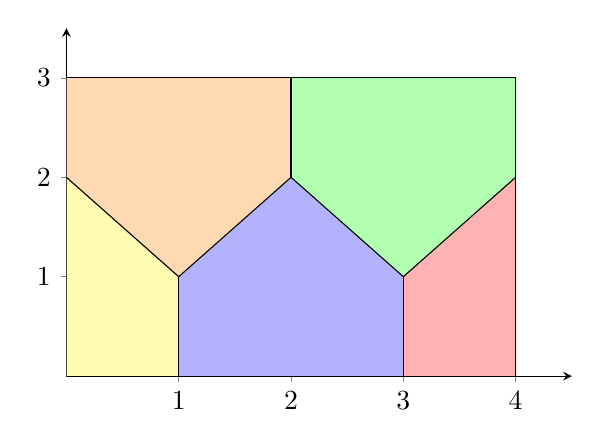
\begin{tikzpicture}
                \begin{axis}[
                    width=8cm, height=6 cm,
                    axis lines = center,
                    axis line style = {},
                     xmin = 0, xmax = 4.5,
                     ymin = 0, ymax = 3.5,
                     xtick = {0,...,5}, 
                     ytick = {0,...,5}, 
                ]
                \filldraw[yellow!30] (1,0) -- (1,1) -- (0,2) -- (0,0) -- cycle;
                \filldraw[blue!30] (1,0) -- (3,0) -- (3,1) -- (2,2) -- (1,1) -- cycle;
                \filldraw[red!30] (3,0) -- (4,0) -- (4,2) -- (3,1) -- cycle;
                \filldraw[green!30] (2,2) -- (3,1) -- (4,2) -- (4,3) -- (2,3) -- cycle;
                \filldraw[orange!30] (0,2) -- (1,1) -- (2,2) -- (2,3) -- (0,3) -- cycle;
                \draw (0,0) rectangle (4,3);
                \draw[black] (0,2) -- (1,1) -- (2,2) -- (3,1) -- (4,2);
                \draw[black] (1,1) -- (1,0);
                \draw[black] (2,2) -- (2,3);
                \draw[black] (3,1) -- (3,0);
                \end{axis}
            \end{tikzpicture}
            \caption{An illustration of E4 part (c)}
            \label{fig:E4c}
        \end{figure}
    \end{enumerate}

\subsection*{\Exercise}
    \textit{(PHP: Dogfighting Tactics) } These problems are a bit more tricky. When we say `plane', we mean a flat, two-dimensional surface, not an airplane ;) Again, show your work.
    \begin{enumerate}
        \item A plane is colored using four colors. Prove that there exist two identically colored points on this plane that are an integer number of inches apart. % Next year, say that all five points cannot be collinear, so the solution cannot just be "draw a straight line"
        \item Place six circles in the plane so that no one of them contains the center of another. Prove that the six circles cannot have a point in common.
        
        \vspace{1mm} \textit{Hint: Suppose there is such a point. Consider drawing lines from the centers to this shared point.}
        \item There are eight lines on the plane. If every line must intersect every other line, prove that some pair of lines forms an angle less than $23^{\circ}$.
        
        \vspace{1mm} \textit{Hint: Try drawing different configurations by hand. What changes if you translate any line in a given configuration?}
    \end{enumerate}

\subsection*{Solution}
    \begin{enumerate}
        \item Without loss of generality, suppose the plane is colored using magenta, cyan, green, and red.
        
        \vspace{1mm}
        On the plane, draw a rectangle of side lengths 6 and 8 inches, as shown in Figure \ref{fig:E5a} (note that the diagonal must be of length 10 inches). Place a point on each of the vertices of the rectangle. Then put another point directly in the center of the rectangle. Since there are four colors (our pigeonholes), but five points (our pigeons), at least two points must share a color. We have chosen the points such that all distances between any pair of points is an integer number of inches, so our proof is complete.
        \begin{figure}[htbp]
        \centering
        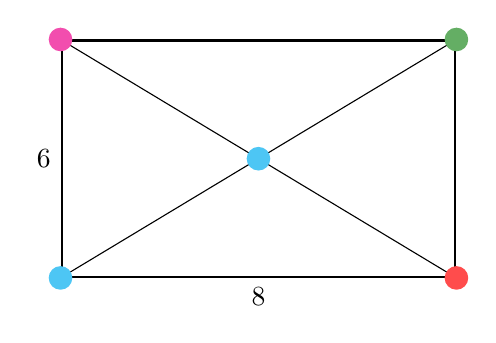
\begin{tikzpicture}[
            roundnode/.style={circle, very thick, minimum size=3mm, inner sep=0pt}]
            % Rectangle with labeled edges
            \node[rectangle, thick, draw, minimum width=50mm, minimum height = 30mm] (R) {};
            
            \draw[black] (R.north west) -- (R.center);
            \draw[black] (R.north east) -- (R.center);
            \draw[black] (R.south west) -- (R.center);
            \draw[black] (R.south east) -- (R.center);
            
            \node[roundnode, fill=magenta!70] at (R.north west) {};
            \node[roundnode, fill=ForestGreen!70] at (R.north east) {};
            \node[roundnode, fill=cyan!70] at (R.south west) {};
            \node[roundnode, fill=red!70] at (R.south east) {};
            \node[roundnode, fill=cyan!70] at (R.center) {};
            
            \node[below] at (R.south) {$8$};
            \node[left] at (R.west) {$6$};
        \end{tikzpicture}
        \caption{Illustration of E5 part (a)}
        \label{fig:E5a}
        \end{figure}
        \item Assume there is a common point $O$ to the six circles. Consider the star made by the centers of each circle connected to the common point. More precisely, if we draw the segments $OC_i$, where $C_{i}$ is the center of the $i$-th circle, then there are six angles $\angle C_iOC_{i+1}$, adding up to $360^{\circ}$. The smallest angle is $\ge 360^{\circ} / 6 = 60^{\circ}$ (this is the pigeonhole application!). After rotation of the labels, we can say that $\angle C_1OC_{2}$ is the smallest angle, with $|OC_1| \ge |OC_2|$.
        
        \vspace{1.5mm}
        Let $\theta = \angle C_1OC_{2}$, $a = |OC_{1}|$, $b = |OC_{2}|$, and $c = C_{1}C_{2}$, the line segment connecting $C_{1}$ and $C_{2}$. Now by the law of cosines, $$c^{2} = a^{2} + b^{2} - 2ab\cos(\theta).$$ Noting that $0 \le \theta \le 60^{\circ}$, $$c^{2} = a^{2} + b^{2} - 2ab\cos(\theta) \le a^{2} + b^{2} - 2ab\frac{1}{2} = a^{2} + b^{2} - ab.$$
        Simplifying this expression is a little tricky. We know $a + b > a$, so $(a - b)(a + b) > a(a - b)$, so $a^{2} - b^{2} > a^{2} - ab$. Finally, we obtain the result $$c^{2} = a^{2} + b^{2} - ab < a^{2} + b^{2} - b^{2} = a^{2} \implies c < a.$$
        
        
        This means that the distance between the two centers is less than the radius of the larger circle, so the larger circle contains the center of the smaller circle. This is a contradiction, therefore the six circles cannot have a point in common.
        \item \qquad We instead prove the slightly stronger statement ``If every line must intersect every other line, prove that some pair of lines forms an angle of length at most $\frac{180}{8} < 23^{\circ}$."
        
        \vspace{1.5mm}
        \qquad Choose one of the eight lines, call it $\ell$. Denote $\alpha_{\ell, i}$ as the angle created by moving counterclockwise from $\ell$ to $i$, where $i$ is one of the other seven lines. If any $\alpha_{\ell, i}$ is at most $\frac{180}{8}$ degrees, then we are done. Otherwise, every $\alpha_{\ell, i}$ is between $180 \cdot \frac{1}{8}$ and $180 \cdot \frac{7}{8}$. Now divide the interval $[180 \cdot \frac{1}{8}, 180 \cdot \frac{7}{8}]$ into six intervals of equal length $\frac{180}{8}$. These are our six pigeonholes, and the seven angles $\alpha_{\ell, i_{1}}, \dots, \alpha_{\ell, i_{7}}$ are our pigeons. Using the pigeonhole principle, for two angles $\alpha_{1}, \alpha_{2} \in \{\alpha_{\ell, i_{1}}, \dots, \alpha_{\ell, i_{7}}\}$, we have $\alpha_{1} - \alpha_{2} \le \frac{180}{8}$, meaning that the angle $\alpha$ created by the corresponding two lines is at most $\frac{180}{8}$, and thus our proof is complete.
        
        \vspace{1.5mm}
        \qquad Figure \ref{fig:E5ca} demonstrates our proof applied to three lines, where we find some $\alpha \le \frac{180}{3} = 60^{\circ}$. Figure \ref{fig:E5cb} demonstrates the case when we have an angle of length exactly $\frac{180}{8}$.
        
        \begin{figure}[htbp]
            \centering
            \begin{subfigure}{0.45\textwidth}
                \centering
                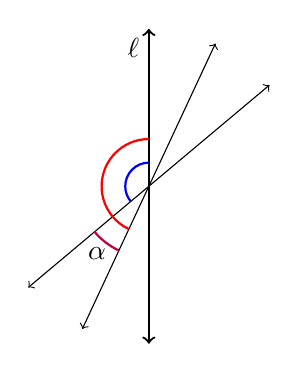
\begin{tikzpicture}
                    \draw[<->, thick] (0,-2) coordinate(A) -- (0,2) coordinate(B);
                    \draw[rotate = 130, <->] (0,-2) coordinate(C) -- (0,2) coordinate(D);
                    \draw[rotate = 155, <->] (0,-2) coordinate(E) -- (0,2) coordinate(F);
                    \node (i) at (0,0) {};
                    \node[below left] at (0, 2) {$\ell$};
                    \path (B) -- (i) -- (D) 
                        pic[draw=blue, thick, angle eccentricity=1.2,angle radius=3mm] {angle=B--i--D};
                    \path (B) -- (i) -- (F) 
                        pic[draw=red, thick, angle eccentricity=1.2,angle radius=6mm] {angle=B--i--F};
                    \path (D) -- (i) -- (F) 
                        pic["$\alpha$", draw=purple, thick, angle eccentricity=1.2,angle radius=9mm] {angle=D--i--F};
                \end{tikzpicture}
                \caption{Our proof applied to $3$ lines.}
                \label{fig:E5ca}
            \end{subfigure}
            \begin{subfigure}{0.45\textwidth}
                \centering
                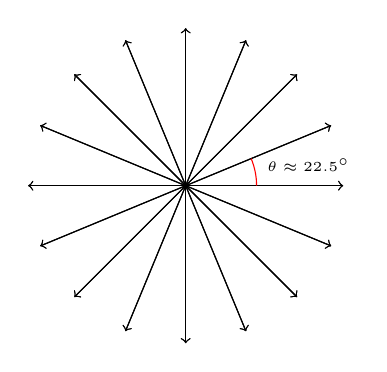
\begin{tikzpicture}
                    \foreach \i in {0,1,...,15}{
                        \draw[rotate = \i * 360/16, <->] (-2, 0) coordinate(n\i a)-- (2, 0) coordinate(n\i b);
                    }
                    \coordinate (O) at (0,0);
                    \path (n0b) -- (O) -- (n9a) 
                        pic["\tiny $\theta \approx 22.5^{\circ}$",draw=red,angle eccentricity=1.2,angle radius=.9cm, pic text options={shift={(5mm,.5mm)}}] {angle=n0b--O--n9a};
                \end{tikzpicture}
                \caption{All eight lines are evenly spaced.}
                \label{fig:E5cb}
            \end{subfigure}
            \caption{Illustration of E5 part (c)}
            \label{fig:E5c}
        \end{figure}
        
    \end{enumerate}

\subsection*{\Exercise}
    \textit{(Swing for the Fences)} You return to The Farm to visit your favorite cow, Pomarrosa. Unfortunately, the farmer informs you that Pomarrosa has escaped, and is now running through the farmland! Luckily, you devise a plan to catch Pomarrosa. 
    
    \vspace{1.5mm}
    Let $m, n, p, q, x, y$ be positive integers. 
    \begin{itemize}
        \item The total farmland can be represented as a $m \times n$ grid.
        \item Pomarrosa is currently eating grass inside the box that is situated at the intersection of the $p$-th row and $q$-th column of the farmland.
        \item While Pomarrosa is eating grass, you and the farmer will quickly enclose her inside an $x \times y$ rectangular fence, where $1 \le x \le m$ and $1 \le y \le n$.
    \end{itemize}
    How many possible fences can you and the farmer build that will enclose Pomarrosa?

\subsection*{Solution}
    The rectangular fence can be defined by its upper left and lower right vertices. 
    
    \vspace{1mm}\qquad To contain Pomarrosa, the upper left vertex must be in a row with a number less than or equal to $p$ and in a column with a number less than or equal to $q$. Thus there are $p \times q$ different positions for the upper left vertex. 
    
    \vspace{1mm}\qquad On the other hand, the lower right vertex must be in a row and column with a number greater than or equal to $p$ and $q$, respectively. Thus there are $(m - p + 1) \times (n - q + 1)$ different positions for the lower right vertex. In conclusion, there are $p \times q \times (m - p + 1) \times (n - q + 1)$ fences containing Pomarrosa.

\end{document}